\documentclass[12pt, letterpaper]{article}

% ============================================
% PAQUETE APA 7 - CONFIGURACIÓN PRINCIPAL
% ============================================
\usepackage[utf8]{inputenc}
\usepackage[spanish]{babel}

% Paquete para formato APA 7
\usepackage[style=apa, backend=biber, language=spanish]{biblatex}
\addbibresource{bibliografia.bib}

% Paquetes matemáticos
\usepackage{amsmath}
\usepackage{amsfonts}
\usepackage{amssymb}

% Paquetes de gráficos y tablas
\usepackage{graphicx}
\usepackage{float}
\usepackage{booktabs}
\usepackage{array}
\usepackage{multirow}
\usepackage{caption}
\usepackage{subcaption}

% Código R
\usepackage{listings}
\usepackage{xcolor}

% ============================================
% CONFIGURACIÓN APA v7: MÁRGENES Y ESPACIADO
% ============================================
\usepackage{geometry}
\geometry{
    letterpaper,
    top=2.54cm, % 1 pulgada (APA v7)
    bottom=2.54cm, % 1 pulgada (APA v7)
    left=2.54cm, % 1 pulgada (APA v7)
    right=2.54cm % 1 pulgada (APA v7)
}

% Doble espaciado (APA v7)
\usepackage{setspace}
\doublespacing

% ============================================
% CONFIGURACIÓN APA v7: ENCABEZADOS Y PIE DE PÁGINA
% ============================================
\usepackage{fancyhdr}
\pagestyle{fancy}
\fancyhf{} % Limpiar encabezados

% Running head (encabezado corto) - Solo en portada
\fancyhead[L]{} % Se configurará después para páginas normales
\fancyhead[R]{\thepage} % Número de página arriba a la derecha (APA v7)

% Línea del encabezado
\renewcommand{\headrulewidth}{0pt} % Sin línea (APA v7)

% ============================================
% CONFIGURACIÓN APA v7: TÍTULOS Y SECCIONES
% ============================================
\usepackage{titlesec}

% Nivel 1: Centrado, Negrita, Capitalizado
\titleformat{\section}
{\normalfont\large\bfseries\centering}{\thesection}{1em}{}

% Nivel 2: Alineado a la izquierda, Negrita
\titleformat{\subsection}
{\normalfont\normalsize\bfseries\raggedright}{\thesubsection}{1em}{}

% Nivel 3: Alineado a la izquierda, Negrita, Cursiva
\titleformat{\subsubsection}
{\normalfont\normalsize\bfseries\itshape\raggedright}{\thesubsubsection}{1em}{}

% ============================================
% CONFIGURACIÓN DE CÓDIGO R
% ============================================
\lstset{ language=R, basicstyle=\ttfamily\footnotesize, commentstyle=
\color{gray}
, keywordstyle=
\color{blue}
, stringstyle=
\color{red}
, showstringspaces=false, breaklines=true, frame=single, backgroundcolor=
\color{gray!10}
}

% ============================================
% CONFIGURACIÓN DE HIPERENLACES
% ============================================
\usepackage{hyperref}
\hypersetup{
    colorlinks=true,
    linkcolor=black, % Enlaces internos en negro (APA prefiere)
    filecolor=black,
    urlcolor=blue, % URLs en azul
    citecolor=black, % Citas en negro (APA)
    pdfborder={0 0 0}
}

% ============================================
% CONFIGURACIÓN APA v7: SANGRÍA DE PÁRRAFO
% ============================================
\setlength{\parindent}{1.27cm} % 0.5 pulgadas (APA v7)

% ============================================
% INFORMACIÓN DEL DOCUMENTO (para portada APA)
% ============================================
\newcommand{\runtitulo}{Análisis de Regresión Lineal}
\newcommand{\titulo}{Análisis de Regresión Lineal Simple: Relación entre Peso y Rendimiento
en el Dataset mtcars}
\newcommand{\autores}{Alisson Atupaña, Mario Camacho, Lenin Lopez}
\newcommand{\afiliacion}{Universidad Nacional de Chimborazo}
\newcommand{\facultad}{Facultad de Ingeniería}
\newcommand{\carrera}{Ciencia de Datos e IA}
\newcommand{\materia}{Modelamiento}
\newcommand{\docente}{Estalin Mejia H.}
\newcommand{\semestre}{Tercero}
\newcommand{\ciudad}{Riobamba - Ecuador}

\begin{document}
    % ============================================
    % PORTADA APA v7
    % ============================================
    \begin{titlepage}
        \thispagestyle{fancy}
        \fancyhf{} \fancyhead[R]{\thepage}

        \centering

        
        \vspace{0.5cm}
        \begin{figure}[H]
            \centering
            
\includegraphics[width=1\linewidth]{Graficos/Imagen1.png}
        \end{figure}
        
        % Título (doble espaciado, negrita, centrado)
        {\Large\bfseries \titulo \par}

        \vspace{2cm}

        % Nombre de los autores
        {\large \autores \par}

        \vspace{0.5cm}

        % Afiliación institucional
        {\large \afiliacion \par} {\normalsize \facultad \par}
        {\normalsize \carrera \par}

        \vspace{1cm}

        % Información del curso
        {\normalsize \textbf{Materia:} \materia \par}
        {\normalsize \textbf{Docente:} \docente \par}
        {\normalsize \textbf{Semestre:} \semestre \par}

        \vfill

        % Fecha y lugar
        {\normalsize \ciudad \par} {\normalsize \today \par}
    \end{titlepage}

    % ============================================
    % CUERPO DEL DOCUMENTO
    % ============================================
    \newpage
    \setcounter{page}{2}

    \section{Introducción}

    \subsection{Planteamiento del Problema}

    Existe una correlación entre el peso de un camión y en su rendimiento en el consumo de combustible constituye un aspecto esencial dentro de la industria automotriz moderna. Diversos investigadores sostienen que la cantidad de peso en la carga influye de manera directa en el rendimiento energético  del vehículo, lo que quiere decir que entre mayor sea el peso, mayor será el consumo del combustible.

    \subsection{Preguntas de Investigación}

    \begin{enumerate}
        \item ¿Existe una relación estadísticamente significativa entre el peso del
            vehículo y su rendimiento de combustible?

        \item ¿Cuál sería el rendimiento de combustible estimado para un vehículo
            sin carga (peso teórico igual a cero)?
    \end{enumerate}

    \subsection{Objetivos}

    \subsubsection{Objetivo General}

 Analizar  la existencia y magnitud de la relación entre el peso del vehículo
    y su rendimiento de combustible mediante un modelo de regresión lineal simple haciendo uso del dataset \texttt{mtcars}.

    \subsubsection{Objetivos Específicos}
    
    \begin{enumerate}
        \item Evaluar la normalidad de las variables mediante pruebas estadísticas
            apropiadas.

        \item Calcular el coeficiente de correlación de Pearson entre el  peso y el rendimiento.

        \item Ajustar un modelo de regresión lineal simple y evaluar su significancia
            estadística.

        \item Validar el cumplimiento de los supuestos del modelo de regresión.

    \end{enumerate}

    \subsection{Hipótesis}

    \textbf{Hipótesis nula ($H_{0}$):} No existe relación una relación lineal significativa entre
    el peso del vehículo y su rendimiento de combustible $H_0: \beta_{1} = 0$

    \textbf{Hipótesis alternativa ($H_{1}$):} Existe una relación lineal significativa
    entre el peso del vehículo y su rendimiento de combustible $H_1: \beta_{1} \neq 0$

    Donde $\beta_{1}$ representa el coeficiente de regresión (pendiente) el cual mide el efecto del peso sobre el rendimiento. Para la prueba de hipótesis se empleará  un nivel de significancia de 
    $\alpha = 0.05$ para el contraste de hipótesis.

    \section{Resultados}

    Se efectuó un análisis estadístico a travez de una metodología lineal desarrollada en seis etapas claves, que se se detallaran junto a los resultados obtenidos de dicho proceso estadístico.
    
    \subsection{Exploración del dataset}

    Consistió en la carga de todo el conjunto de datos empleados desde el dataset \texttt{mtcars}, que contiene información 
    sobre 32 vehículos publicada por  la revista \textit{Motor Trend} de 1974, disponible
    en el entorno estadístico R \parencite{rcore2023}. Dicho dataset contiene 11 variables de las cuales fueron seleccionadas las mas relevantes para dicho analisis:

    \begin{itemize}
        \item \textbf{mpg} (Miles Per Gallon): Hace referencia al rendimiento de combustible, y se ha asignada
            como la variable dependiente.
        \item \textbf{wt} (Weight): Hace referencia al peso del vehículo expresado en miles de libras,
            asignada como la variable independiente.
    \end{itemize}

    El beneficio de la exploracion reveló que el dataset no contiene valores faltantes (\textit{N/A}) en ninguna de las dos variables de interés, lo que permitio proceder al calculo sin usar procedimientos de eliminacion o relleno de datos en las observaciones, la siguiente tabla \ref{tab:estructura} resume la estructura del dataset.

    \begin{table}[H]
        \centering
        \caption{Estructura y Completitud del Dataset mtcars}
        \begin{tabular}{@{}lccc@{}}
            \toprule 
            \textbf{Variable} & \textbf{Observaciones} & \textbf{Valores Perdidos} & \textbf{Completitud} \\
            \midrule 
            Rendimiento (mpg) & 32 & 0 & 100\% \\
            Peso (wt)         & 32 & 0 & 100\% \\
            \midrule
            \textbf{Total}    & 32 & 0 & 100\% \\
            \bottomrule
        \end{tabular}
        \label{tab:estructura}
        
        \vspace{0.2cm}
        \textit{Nota.} El dataset no requiere tratamiento de valores perdidos. Todas las 
        observaciones están completas para ambas variables de estudio.
    \end{table}

    \subsection{Cálculo de Estadísticas Descriptivas}

    Se hizo enfasis al cálculo de medidas de tendencia central, como la dispersión
    y rango, que se realizó para observar las estadísticas de las dos variables. La Tabla \ref{tab:descriptivas}
    resume estos estadísticos descriptivos.

    \begin{table}[H]
        \centering
        \caption{Estadísticas Descriptivas de las Variables de Estudio}
        \begin{tabular}{@{}lcccccc@{}}
            \toprule 
            \textbf{Variable} & \textbf{Media} & \textbf{Mediana} & \textbf{DE} & \textbf{Mín} & \textbf{Máx} & \textbf{n} \\
            \midrule 
            Rendimiento (mpg) & 20.09          & 19.20            & 6.03        & 10.40        & 33.90        & 32         \\
            Peso (1000 lbs)   & 3.22           & 3.33             & 0.98        & 1.51         & 5.42         & 32         \\
            \bottomrule
        \end{tabular}
        \label{tab:descriptivas}
        
        \vspace{0.2cm}
        \textit{Nota.} DE = Desviación Estándar; Mín = Mínimo; Máx = Máximo; n = Tamaño de muestra.
    \end{table}

    \begin{figure}[H]
        \centering
        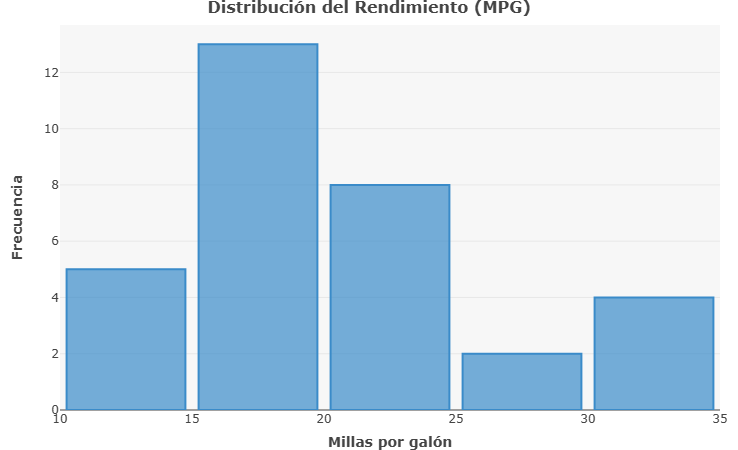
\includegraphics[width=0.45\textwidth]{Graficos/distribuicion del rendimiento.png}
        \hfill
        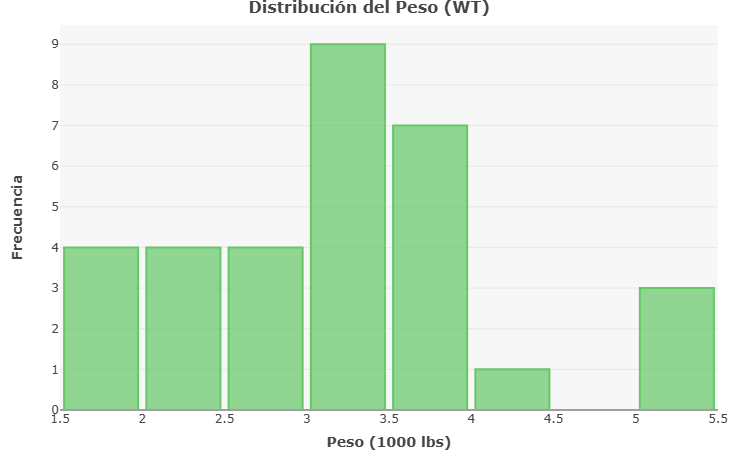
\includegraphics[width=0.45\textwidth]{Graficos/distribuicion del peso.png}
        \caption{Histogramas de las variables de estudio}
        \label{fig:histogramas}
    \end{figure}

    Por lo tanto se detallan los hallazgos mostrados en la tabla anterior:

    \begin{itemize}
        \item El rendimiento promedio de los vehículos es de 20.09 mpg con una
            desviación estándar de 6.03 mpg, lo que evidencia una variabilidad notable 
            en la eficiencia del consumo de combustible.
        \item El peso promedio de los vehículos es de 3.22 miles de libras, que equivale a (3,220 lbs)
            con una desviación estándar de 0.98 miles de libras.
        \item El rendimiento varia entre 10.40 mpg (vehículo menos eficiente)
 y 33.90 mpg (vehículo más eficiente), reflejando  una diferencia
            superior al triple.
        \item El rango de peso de los vehículos oscila  entre  1.51 miles de libras (vehículo más ligero)
            y 5.42 miles de libras (vehículo más pesado).
        \item La escasa diferencia entre la media y la mediana en ambas variables sugiere que sus distribuciones son relativamente simétricas. 
    \end{itemize}

    \subsection{Proceso de Normalidad de las Variables}

    Consistió en evaluar si las variables se encuentran en una distribución normal, un requisito indispensable para verificar la validez de las inferencias en la regresión lineal. Ademas, se aplicó una prueba de Shapiro-Wilk \textcite{shapiro1965}, cuya hipótesis nula define que los datos tienen un origen de una distribución normal.

    \begin{table}[H]
        \centering
        \caption{Resultados de la Prueba de Normalidad de Shapiro-Wilk}
        \begin{tabular}{@{}lccc@{}}
            \toprule 
            \textbf{Variable}     & \textbf{Estadístico W} & \textbf{p-valor} & \textbf{Decisión ($\alpha = 0.05$)} \\
            \midrule 
            Rendimiento (mpg)     & 0.9475                 & 0.1229           & No se rechaza $H_0$ (Normal)       \\
            Peso (1000 lbs)       & 0.9269                 & 0.0473           & Se rechaza $H_0$ (No normal)       \\
            \bottomrule
        \end{tabular}
        \label{tab:normalidad}
        
        \vspace{0.2cm}
        \textit{Nota.} Nivel de significancia: $\alpha = 0.05$. El estadístico W cercano a 1 indica mayor normalidad.
    \end{table}

    \newpage
    Dichos resultados dan a indicar que:

    \begin{itemize}
        \item \textbf{Variable rendimiento (mpg):} Con $W = 0.9475$ y $p = 0.1229 > 0.05$, se efectua que no se rechaza la hipótesis nula, por lo tanto permite concluir que el rendimiento sigue una distribución medianamente normal.
        \item \textbf{Variable peso (wt):} Con $W = 0.9269$ y $p = 0.0473 < 0.05$, da a entender que
            se rechaza la hipótesis nula, concluyendo en una ligera desviación de la
            normalidad.
    \end{itemize}

    

    \subsection{Cálculo de la Correlación de Pearson}

    Este cálculo es importante porque permite determinar si existe una asociación lineal antes de proceder al ajuste del modelo de regresión. Por lo tanto, se le aplicó la prueba de correlación de Pearson con las siguientes hipótesis:
    \begin{itemize}
        \item $H_0$: No existe correlación lineal entre peso y rendimiento ($\rho = 0$)
        \item $H_1$: Existe correlación lineal entre peso y rendimiento ($\rho \neq 0$)
    \end{itemize}

    Una vez establecido esto, los resultados del anterior análisis de Pearson son:

    \begin{table}[H]
        \centering
        \caption{Resultados del Análisis de Correlación de Pearson}
        \begin{tabular}{@{}lc@{}}
            \toprule 
            \textbf{Estadístico} & \textbf{Valor} \\
            \midrule 
            Coeficiente de correlación ($r$) & $-0.868$ \\
            Estadístico $t$ & $-9.559$ \\
            Grados de libertad & 30 \\
            p-valor & $< 0.001$ \\
            Intervalo de confianza 95\% & $[-0.934, -0.744]$ \\
            \bottomrule
        \end{tabular}
        \label{tab:correlacion}
    \end{table}

    \begin{figure}[H]
        \centering
        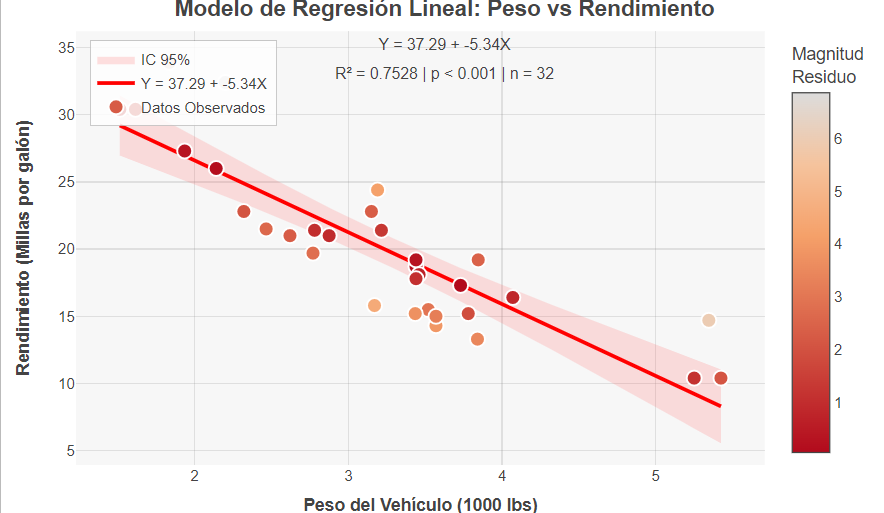
\includegraphics[width=0.75\textwidth]{Graficos/Grafico ajustado.png}
        \caption{Gráfico de dispersión: Relación entre peso y rendimiento con línea de regresión ajustada}
        \label{fig:dispersion}
    \end{figure}

    \begin{itemize}
        \item El coeficiente con un valor de $r = -0.868$ indica una correlación lineal
            \textbf{negativa, ademas de fuerte} entre peso del camión y el rendimiento de combustible. Ademas, el signo negativo
            afirma que a mayor peso la carga, menor rendimiento en el combustible.
        \item El p-valor de $< 0.001$ da la capacidad de rechazar la hipótesis nula con un nivel
            de confianza superior al 99.9\%, lo que confirma que la correlación es muy significativa.
        \item Con un intervalo de confianza al 95\% ($[-0.934, -0.744]$), da un refuerzo de que la correlación es negativa para la población.
        \item Finalmente, el estadístico da como $t = -9.559$ asignados a 30 grados de libertad indica que es altamente
            significativo, por lo que da a entender que la correlación observada es muy improbable
            bajo la hipótesis nula.
    \end{itemize}
    

    \subsection{Ajuste del Modelo de Regresión Lineal Simple}

    Se ajustó el modelo de regresió lineal simple usando un metodo de minimos cuadrados ordinarios, que permite estimar los coeficientes $\beta_0$ (intercepto) y $\beta_1$ (pendiente) minimizando la suma de los cuadrados de los residuos. Por lo tanto, el modelo ajustado es expresado mediante la siguiente ecuación:

    \begin{equation}
        \widehat{\text{mpg}} = 37.285 - 5.344 \times \text{wt}
        \label{eq:modelo}
    \end{equation}

    \subsubsection{Estimación de los Coeficientes}

    En la siguiente tabla se presenta los coeficientes que se han estimados en el modelo junto a sus errores estandares, asi como estadisticos de pruebas y valores p.

    \begin{table}[H]
        \centering
        \caption{Coeficientes del Modelo de Regresión Lineal Simple}
        \begin{tabular}{@{}lcccc@{}}
            \toprule 
            \textbf{Coeficiente}       & \textbf{Estimación} & \textbf{EE} & \textbf{Estadístico t} & \textbf{p-valor} \\
            \midrule 
            $\beta_{0}$ (Intercepto)   & 37.285              & 1.878       & 19.858                 & $< 0.001$        \\
            $\beta_{1}$ (Peso)         & $-5.344$            & 0.559       & $-9.559$               & $< 0.001$        \\
            \bottomrule
        \end{tabular}
        \label{tab:regresion}
        
        \vspace{0.2cm}
        \textit{Nota.} EE = Error Estándar. Los estadisticos t se calcularon como: $t = \frac{\hat{\beta}_i}{EE(\hat{\beta}_i)}$.
    \end{table}

    \begin{enumerate}
        \item \textbf{Intercepto ($\beta_0 = 37.285$ mpg):}
        \begin{itemize}
            \item Es el valor predicho al rendimiento cuando el peso es cero
                ($wt = 0$).
            \item Por lo tanto es estadísticamente significativo ($t = 19.858$, $p < 0.001$).
        \end{itemize}

        \item \textbf{Pendiente ($\beta_1 = -5.344$ mpg por 1000 lbs):}
        \begin{itemize}
            \item Estima el cambio esperado en el rendimiento por cada aumento
                de en las unidades de peso.
            \item El signo negativo confirma la relación inversa: a mayor peso, menor
                rendimiento.
            \item Por lo tanto es altamente significativo ($t = -9.559$, $p < 0.001$), lo que permite rechazar
                la hipótesis nula $H_0: \beta_1 = 0$.
            \item Finalmente el error estándar de 0.559 da a entender que tiene una alta precisión en la estimación
                del coeficiente.
        \end{itemize}
    \end{enumerate}

    \subsubsection{Evaluación de la Bondad de Ajuste}

    Para probar la calidad del modelo ya ajustado se calculo multiples metricas de bondad de ajuste:

    \begin{table}[H]
        \centering
        \caption{Metricas de Bondad de Ajuste del Modelo}
        \begin{tabular}{@{}lc@{}}
            \toprule 
            \textbf{Métrica} & \textbf{Valor} \\
            \midrule 
            Coeficiente de determinación ($R^{2}$) & 0.7528 \\
            Error estándar residual (RSE) & 3.046 mpg \\
            Estadístico F & 91.375 \\
            Grados de libertad & (1, 30) \\
            p-valor (prueba F) & $< 0.001$ \\
            \bottomrule
        \end{tabular}
        \label{tab:bondad}
    \end{table}

    \begin{itemize}
        \item \textbf{$R^{2} = 0.7528$:} El coeficiente de determinación nos muestra que
            el 75.28\% de la variabilidad total observada en el rendimiento del combustible puede atribuirse al peso del vehículo. Este resultado refleja un nivel de ajuste sobresaliente para un modelo de regresión lineal simple, lo que confirma que el peso  es
            un predictor muy relevante del rendimiento.

        \item \textbf{Error estándar residual = 3.046 mpg:} Nos indica que las diferencias promedio entre los valores reales y los valores predichos por el modelo son de aproximadamente 3.05 millas por galón. Es decir, las predicciones realizadas presentan una precisión adecuada. 

        \item \textbf{Prueba F global:} Con $F_{1,30} = 91.375$ y $p < 0.001$, se
            rechaza la hipótesis nula, la cual plantea que todos los coeficientes de regresión  (excepto
            el intercepto) son cero. Esto confirma que el modelo en su conjunto es
            estadísticamente significativo y tiene capacidad predictiva real.
    \end{itemize}

    \subsubsection{Normalidad de los Residuos}

    \textbf{Método de verificación:} Prueba de Shapiro-Wilk aplicada a los residuos
    y análisis del gráfico Q-Q (cuantiles teóricos versus observados).

    \begin{table}[H]
        \centering
        \caption{Prueba de Normalidad de los Residuos (Shapiro-Wilk)}
        \begin{tabular}{@{}lc@{}}
            \toprule 
            \textbf{Estadístico} & \textbf{Valor} \\
            \midrule 
            Estadístico W & 0.946 \\
            p-valor & 0.279 \\
            \bottomrule
        \end{tabular}
        \label{tab:normalidad_residuos}
    \end{table}

    \textbf{Resultado:} Dado que el estadístico obtenido fue  $W = 0.946$ y $p = 0.279 > 0.05$, no se rechaza la
    hipótesis nula de normalidad. Ademas, el grafico Q-Q mostró que los residuos se ajustan 
    razonablemente bien con la línea diagonal teórica, con desviaciones mínimas en
    los extremos.

    \textbf{Conclusión:} El supuesto de normalidad de los residuos se cumple
    satisfactoriamente.

    \begin{figure}[H]
        \centering
        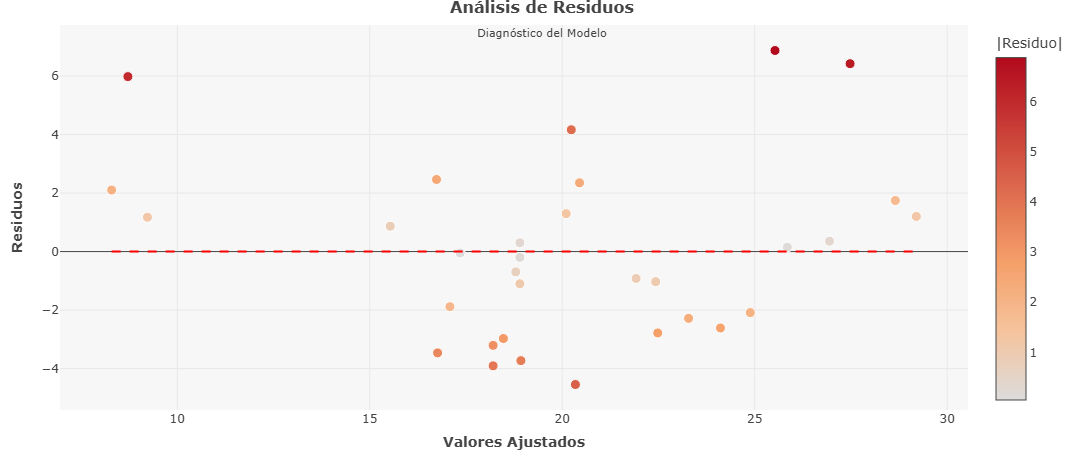
\includegraphics[width=0.8\textwidth]{Graficos/analisis de residuos.png}
        \caption{Gráficos de diagnóstico del modelo: Residuos vs. Valores ajustados}
        \label{fig:diagnostico}
    \end{figure}

 
    \subsection{Generación de Predicciones}

    El septimo y último paso consisti en aplicar el modelo de regresión  validado para estimar
    el rendimiento del combustible para diferentes valores de peso.
    Este procedimiento permitió responder a las preguntas practicas de la investigación y demostrar la utilidad predicha del modelo obtenido.    

    \subsubsection{Metodologia de Prediccion}

    Las predicciones se generaron utilizando la ecuación del modelo (Ecuación \ref{eq:modelo}):
    \begin{equation*}
        \widehat{\text{mpg}} = 37.285 - 5.344 \times \text{wt}
    \end{equation*}

    Se seleccionaron valores de peso que abarcan tanto el rango observado en los
    datos (1.51 a 5.42 miles de libras)  ademas de incluir una extrapolación al caso teórico de
    peso cero, con el propósito de responder directamente a una de las preguntas de investigación
    formuladas.

    \subsubsection{Resultados de las Predicciones}

    \begin{table}[H]
        \centering
        \caption{Predicciones de Rendimiento según Peso del Vehículo}
        \begin{tabular}{@{}ccc@{}}
            \toprule 
            \textbf{Peso (1000 lbs)} & \textbf{Rendimiento Predicho (mpg)} & \textbf{Tipo de Predicción} \\
            \midrule 
            0.0*                     & 37.29                               & Extrapolación              \\
            1.5                      & 29.27                               & Interpolación              \\
            2.0                      & 26.60                               & Interpolación              \\
            2.5                      & 23.92                               & Interpolación              \\
            3.0                      & 21.25                               & Interpolación              \\
            3.5                      & 18.58                               & Interpolación              \\
            4.0                      & 15.91                               & Interpolación              \\
            4.5                      & 13.24                               & Interpolación              \\
            5.0                      & 10.56                               & Interpolación              \\
            \bottomrule
        \end{tabular}
        \label{tab:predicciones}
        
        \vspace{0.2cm}
        \textit{Nota.} *El valor de peso = 0 está fuera del rango observado (1.51-5.42 miles de libras) 
        y constituye una extrapolación teórica. Las predicciones de interpolación son más confiables.
    \end{table}

    \subsubsection{Interpretacion de las Predicciones}

    \begin{enumerate}
        \item \textbf{Predicción para peso cero :}
        Un vehículo hipotético sin carga presentaría  un rendimiento predicho de 37.29 mpg.
        No obstante, esta predicción requiere interpretación cautelosa debido a  tres factores:
        \begin{itemize}
            \item Es una extrapolación fuera del rango de datos observados
            \item No existe un vehículo real con un peso en cero
            \item La relación lineal podría no mantenerse en valores extremos
        \end{itemize}
        Sin embargo, este valor responde teóricamente a la pregunta de investigación planteada y
        representa el intercepto del modelo.

        \item \textbf{Tendencia sistemática:} Las predicciones muestran una disminución
        consistente del rendimiento a medida que  aumenta el peso del vehículo, confirmando la relación
        inversa identificada en el análisis estadístico .

    \end{enumerate}

      \section{Discusion}

    \subsection{Interpretación de los Hallazgos}

El presente análisis se llevo a acabo con el único propósito de evaluar de manera estadística y objetiva la relación existente entre el peso de un vehículo y su rendimiento en el consumo de combustible, las variables fueron consideradas fundamentales dentro del ámbito de la ingeniería automotriz y la eficiencia energética. 

El peso se eligió por su influencia directa en la resistencia al movimiento y el consumo, mientras que el rendimiento (millas por galón ) el cual nos permitió medir de forma cuantitativa la eficiencia del vehículo. 

    Los resultados del análisis proporcionan evidencia sólida que respalda la hipótesis
    de que existe una relación lineal significativa entre el peso del vehículo y
    su rendimiento de combustible. Los principales hallazgos se interpretan de la
    siguiente manera:

    \begin{enumerate}
        \item \textbf{Significancia estadística:} El p-valor inferior a 0.001 permite
            rechazar la hipótesis nula ($H_0: \beta_1 = 0$) con un alto nivel de
            confianza, confirmando que el peso del vehículo es un predictor estadísticamente
            significativo del rendimiento de combustible.

        \item \textbf{Magnitud de la relación:} El coeficiente de correlación de
            Pearson ($r = -0.868$) indica una asociación negativa fuerte entre ambas
            variables. Esto significa que conforme aumenta el peso, el rendimiento
            disminuye de manera consistente y pronunciada.

        \item \textbf{Capacidad explicativa:} El coeficiente de determinación
            ($R^{2} = 0.7528$) revela que el 75.28\% de la variabilidad observada en
            el rendimiento puede ser explicada únicamente por el peso del vehículo,
            lo que constituye un ajuste muy satisfactorio para un modelo de regresión
            simple.

        \item \textbf{Interpretación práctica del modelo:} El coeficiente de regresión
            ($\beta_1 = -5.344$) indica que por cada incremento de 1000 libras en el
            peso del vehículo, se espera una disminución promedio de 5.34 millas por
            galón en el rendimiento. Esta cuantificación precisa del efecto tiene
            implicaciones directas para la eficiencia energética y económica del
            transporte.
    \end{enumerate}

    En conjunto, este procedimiento permitió verificar el impacto del peso en la eficiencia del combustible y proporcionar una base analítica útil para  futuros estudios sobre transporte eficiente.

    \subsection{Respuestas a las Preguntas de Investigación}

    Con base en los resultados obtenidos, se responden las preguntas planteadas
    inicialmente:

    \textbf{Pregunta 1:} ¿Existe una relación estadísticamente significativa entre
    el peso del vehículo y su rendimiento de combustible?

    \textbf{Respuesta:} Sí, existe una relación estadísticamente significativa y
    negativa. El análisis demuestra de manera concluyente que el peso del vehículo
    incide negativamente en su rendimiento de combustible ($\beta_1 = -5.344$,
    $t = -9.559$, $p < 0.001$). La correlación negativa fuerte ($r = -0.868$)
    confirma que vehículos más pesados presentan sistemáticamente un menor rendimiento
    de combustible.

    \textbf{Pregunta 2:} ¿Cuál sería el rendimiento de combustible predicho para
    un vehículo sin carga?

    \textbf{Respuesta:} Según el modelo ajustado, un vehículo hipotético sin carga
    (peso = 0) tendría un rendimiento teórico de 37.29 millas por galón. No obstante,
    esta predicción debe interpretarse con precaución, ya que constituye una
    extrapolación más allá del rango de valores observados en el dataset (peso mínimo:
    1.51 miles de libras). En términos prácticos, esta estimación representa el
    intercepto del modelo y no necesariamente refleja una condición real alcanzable.


    \newpage

    % ============================================
    % REFERENCIAS - APA v7 (Generadas automáticamente desde bibliografia.bib)
    % ============================================
    \section{Referencias}

    % Las referencias se generan automáticamente en formato APA v7
    % desde el archivo bibliografia.bib usando biblatex-apa
    %
    \printbibliography
    [heading=none]

    % NOTA: Para citar en el texto, usa:
    % \textcite{clave} para citas narrativas: "Autor (2020) afirma que..."
    % \parencite{clave} para citas parentéticas: "... (Autor, 2020)"
    % Las referencias aparecerán aquí automáticamente cuando cites en el texto

    \nocite{pearson1896}
    \nocite{henderson1981}
    \nocite{montgomery2012}
    \nocite{james2013}
    \nocite{kutner2005}
    \nocite{anscombe1973}
    \nocite{cohen2003}
    \nocite{breusch1979}
    \nocite{shapiro1965}
    \nocite{fox2016}
    \nocite{rawlings1998}
    
\end{document}